\documentclass[main.tex]{subfiles}
\begin{document}
\chapter{STM32}
\section{Introduzione ai micro ARM e CORTEX}
\begin{itemize}
    \item Sono RISC(reduced instruction set)
    \item 1 colpo di clock ad istruzione(contro i 12 in media dell'8051)
    \item 32 bit
    \item Istruzioni di lunghezza fissata per avere velocità fissa
    \item Ogni operando per essere processato viene prima prelevato dalla memoria e salvato nei registri interni del micro secondo la filosofia Load-Store
    \item Pipeline per poter iniziare ad eseguire un'istruzione prima che sia terminata l'esecuzione dell'ultima istruzione.
\end{itemize}
\subsection{Configurazione del micro}
La configurazione del'STM32 avviene attraverso il programma CUBE MX, il quale propone anche una visualizzazione grafica dei pin della scheda. Al contrario di quanto accadeva con l'8051 per questo micro non è necessario disabilitare il watchdog o tantomeno avere una configurazione comune a tutte le esperienze.
\section{Seriale}
L'esperienza della seriale è del tutto analoga a quella con l'8051, il programma è diviso in 3 fasi:\begin{enumerate}
    \item Nella prima fase si trasmette un messaggio di benvenuto al computer
    \item Nella seconda fase il micro entra in modalità eco, ritrasmettendo indietro tutti i caratteri che gli si mandano
    \item Infine riceve una serie di caratteri memorizzandoli e poi rimandando il messaggio ricevuto
\end{enumerate}
Per la USART è stata usata la USART2 del micro abilitandola dal STM32Cube e se ne è abilitato l'interrupt nel NVIC(Nested Vector Interrupt Controller), questo perché la USART2 è già implementata nell'STLink quindi la comunicazione avviene tramite il cavo mini-USB. 

Un'ulteriore differenza con l'8051 è che il buffer per la trasmissione e per la ricezione sono distinti(il che probabilmente rende più chiaro anche il codice) e sono rispettivamente \textit{TDR} e \textit{RDR}. 

Si è creato un file\_condiviso.h come header sia per il file main.c sia per il file che gestisce gli interrupt(stm32f0xx\_it.c). Esso contiene alcune definizioni importanti per entrambi i codici e permette il dialogo tra i due file, come ad esempio \textit{puntatore} che viene usata da entrambi.
\begin{lstlisting}[language=C,caption=Header dei files]
#define CR 13
#define LF 10
#define ML 10
extern unsigned char * puntatore;
extern unsigned char msg_ricevuto[ML+4];
extern int lenght_da_trasmettere;
extern unsigned char  messaggio_benvenuto[7];
extern int lenght;
extern unsigned char msg_errore[10];
extern int lenght_errore;
extern int status;
extern int i;
extern int loaded;
\end{lstlisting}
Quelle riportate di seguito sono le inizializzazioni delle variabili precedenti nel main.
\begin{lstlisting}[language=c,caption=Inizializzazione variabili]
unsigned char * puntatore;
unsigned char msg_ricevuto[ML+4];
int lenght_da_trasmettere=6;
unsigned char messaggio_benvenuto[]={'C','i','a'
,'o',CR,LF};
unsigned char;
msg_errore[]={CR,LF,'E','r','r','o','r','e',CR,LF};
int lenght_errore=10;
int status = 0;
int loaded =0;
int i=0;
\end{lstlisting}

Il vero codice inizia dopo che è avvenuta la configurazione del micro, abilitando l'interrupt di trasmissione e ricezione della USART2. Successivamente si passa il primo carattere da trasmettere al registro TDR.\footnote{È necessario fare il reset del bit di transmission completed perché quando vengono abilitati gli interrupt il micro entra in interrupt e se questo bit fosse 1 lo interpreterebbe come primo carattere trasmesso}
\begin{lstlisting}[language=C,caption=main]
//reset del interrupt control register
//al bit trasmission completed
USART2->ICR |= USART_ICR_TCCF;
//abilito l'interrupt per la trasmissione
USART2->CR1 |= USART_CR1_TCIE;
//abilito l'interrupt per la ricezione
USART2->CR1 |= USART_CR1_RXNEIE;
//inizio a trasmettere il messaggio di benvenuto
msg_ricevuto[0]=CR;
msg_ricevuto[1]=LF;
puntatore= messaggio_benvenuto;
USART2->TDR=*puntatore;
\end{lstlisting}
Quando il micro finisce di trasmettere entra nell'interrupt con il bit di TC ad 1, a questo punto è necessario fare qualcosa e sarà la funzione scelta a determinare cosa.
\begin{lstlisting}[language=C, caption=gestione dell'interrupt]
if((USART2->ISR & USART_ISR_TC) == USART_ISR_TC){
	//resetto il flag di trasmissione completata
	USART2->ICR |= USART_ICR_TCCF;
	//allora ho appena finito di trasmettere
	scelta();
	loaded=0;
	return;
	}
else if((USART2->ISR&USART_ISR_RXNE)==USART_ISR_RXNE){
	//allora ho appena finito di ricevere
	scelta();
	return;
	}
\end{lstlisting}

La funzione scelta è il cuore di questo programma. È l'evoluzione della stessa implementata per la seriale in C \ref{lst:scelta}.
\begin{lstlisting}[language=C,caption=Funzione scelta,label={lst:scelta_due}]
void scelta(){
	unsigned char carattere;
	switch(status){
		case 0:
			//inserisco nel buffer di trasm il carattere
			i++;
			if(i<lenght_da_trasmettere){
				USART2->TDR=*(puntatore+i);
			}
			else{
				status=1;
				i=0;
			}
			break;
		case 1:
			//do
				//inserisco nel buffer di trasmissione
				//il carattere trovato nel buffer in ricezione
				carattere = (char)USART2->RDR;
				if(carattere=='#'){
					i=2;
					status=2;
				}
				else{
				if(!loaded){
					loaded=1;
					USART2->TDR=carattere;
				}
			}
			break;
		case 2:
			//do
				
				carattere=USART2->RDR;
				if(i<ML+3){
					//aggiungo il carattere letto al vettore
					msg_ricevuto[i]=carattere;
					i++;
					if(carattere=='#'){
						//smetto di ricevere
						status=0;
						puntatore=msg_ricevuto;
						msg_ricevuto[i-1]=CR;
						msg_ricevuto[i]=LF;
						lenght_da_trasmettere=i+1;
						i=0;
						//trasmetto il messaggio ricevuto
						USART2->TDR=*puntatore;
					}
				}
				else{
					status=0;
					//trasmetto il messaggio di errore
					puntatore=msg_errore;
					lenght_da_trasmettere=lenght_errore;
					i=0;
					USART2->TDR=*puntatore;
				}
			
			break;
	}
}
\end{lstlisting}
\section{Timer7 e Led}
Questa esperienza è analoga a quella svolta con il led ed il bottone per l'8051 in C(referenza:\ref{led in C}). Infatti l'obiettivo è di realizzare un programma in cui si possa cambiare la luminosità del LED sfruttando gli interrupt del timer del micro ed il bottone. Dunque è stato configurato il Timer 7(TIM7) a 16 bit e l'overflow a 10000(quindi il timer conta da 0 a 10000), con il relativo interrupt. Abbiamo abilitato la porta PA5 come GPIO output per poter accendere e spegnere il led, ed è stato abilitato l'interrupt esterno della porta PC13(il bottone), di modo che ogni volta che viene premuto, viene generato un interrupt.

La funzione wait\_tim aspetta che il timer abbia raggiunto n interrupt, facendo trascorrere un po' di tempo.
\begin{lstlisting}[language=C, caption=Funzione wait\_tim per aspettare]
void wait_tim(){
	wait=1;
	TIM7->CNT=0;//si imposta il contatore a 0
	TIM7->SR=0;//si imposta lo status register a 0
	//si abilita il counter per iniziare a contare
	TIM7->CR1|=TIM_CR1_CEN;
	//si aspetta fino a che non viene settata a 0
	while(wait){}
}
\end{lstlisting}
All'interno dell'interrupt del timer è necessario fare un check sulla variabile \textit{loop}, la quale indica quanti cicli di interrupt bisogna attendere prima di fermare il timer.  
\begin{lstlisting}[language=C, caption=Gestione dell'interrupt del timer]
if(loops>0){
		loops-=1;
		TIM7->CR1|=TIM_CR1_CEN;
	}
else{
	wait=0;//si puo smettere di aspettare
	//e smettere di contare
	TIM7->CR1&=~TIM_CR1_CEN;
}
\end{lstlisting}

All'interno dell'interrupt del bottone è necessario cambiare la luminosità, questo come nel caso della luminosità in C\ref{lst:led in C}, viene fatto cambiando il numero di loop che il led sta accesso ovvero la variabile \textit{loop\_on}. Come nel caso del C, la variabile status indica 5 possibili luminosità(0,25,50,75,100), ciclando su di essi.
\begin{lstlisting}[language=C, caption=Gestione interrupt del bottone]
if(status<4){
	status++;
}
else{
	status=0;
}
loops_on=n_loops*status*25/100;//cambio la luminosita'
//resetto
wait=0;
acceso=0;
\end{lstlisting}

\begin{lstlisting}[language=C, caption=Variabili globali interrupt]
int status=0;
int loops_on=0;
int n_loops=50;
int acceso;
int wait;
volatile int loops=0;
\end{lstlisting}

\begin{lstlisting}[language=C,caption=Variabili globali main]
extern int loops_on;
extern int n_loops;
extern int acceso;
extern int wait;
extern int loops;
\end{lstlisting}
All'interno del main è necessario innanzitutto abilitare l'interrupt del timer, successivamente si entra in un loop infinito all'interno del quale si continua ad accendere e spegnere il led. Il led rimane acceso per \textit{loops\_on} cicli e spento per \textit{n\_loops-loops\_on} cicli, con \textit{n\_loops} il numero massimo di cicli. 

\begin{lstlisting}[language=C,caption=Main]
//abilito l'interrupt del timer
TIM7->DIER|=TIM_DIER_UIE;
while (1)
  {
	if(acceso==0){
		//accendo
		//cambio lo stato del led
		HAL_GPIO_TogglePin(GPIOA,GPIO_PIN_5);
		//devo aspettare loops_on cicli
		loops=loops_on;
		wait_tim();
		acceso=1;
	}
	else{
		//spengo
		HAL_GPIO_TogglePin(GPIOA,GPIO_PIN_5);
		//devo aspettare loops massimi - loops_on
		loops=n_loops-loops_on;
		wait_tim();
		acceso=0;
	}
}
\end{lstlisting}


\section{I2C, termometro e display}


\subsection{Configurazione del micro}


L'esperienza riguardante il protocollo di trasmissione I2C vede coinvolta, oltre che al micro STM32F072rb, anche una scheda da posizionare sopra la scheda di sviluppo Nucleo, al di sopra della quale è connesso un LCD, un termometro ed una manopola, insieme a 4 led. Obbiettivo dell'esperienza è mettere in comunicazione il micro con il display ed il termometro attraverso l'i2c e leggere il potenziale registrato dalla manopola attraverso l'adc. 
Prima di iniziare a scrivere il codice è stato necessario configurare attraverso CUBE il micro, essendo la scheda posizionata sui pin del nucleo bisogna selezionare i pin adibiti alla comunicazione I2C, quelli per l'ADC e i pin dei led. In particolare le operazioni eseguite sono le seguenti:
\begin{itemize}
    \item Attivare l'I2C1 sui pin PB8 e PB9
    \item Abilitare PA5 come GPIO\_Output, per il reset del display
    \item Abilitare PA9 come GPIO\_Output, per la retroilluminazione del display
    \item Abilitare PC0 e PC3 come GPIO\_Output, servono per il termometro. (Notare che i pin di comunicazione I2C sono gli stessi sia per il display che per il termometro, è una caratteristica intrinseca del protocollo I2C avere solo due linee adibite alla comunicazione multiutente, una per il clock e una per i dati)
    \item Abilitare PA0 come ADC\_IN0 ovvero come porta per l'ADC
    \item Le porte PB0,PB1,PB2,PB3 sono messe come GPIO\_Output per comandare i 4 led
\end{itemize}
È stato ovviamente abilitato l'interrupt dell'ADC, dell'I2C, del Timer7(con un autoreload value di 48000, ovvero parte da 0 e arriva a 48000) in modo che con il clock a 48MHz andasse in overflow ogni 1ms. La frequenza dell'ADC è stata invece impostata a 14MHz.
Per una seconda parte dell'esperienza è stata anche attivata la USART2 come nelle precedenti esperienze(freq. a 9600bit/s...) con il relativo interrupt.


\subsection{Esperienza}

Descrizione del programma I2C display termometro. 
L'obiettivo di questo programma è scrivere su un display la temperatura registrata dal termometro e 
il potenziale registrato da un potenziometro a manopola letto dall'adc.
è necessario dividere il programma in più parti:
\begin{itemize}
    \item Leggere dall'ADC il potenziale
    \item Inizializzare il display
    \item Leggere la temperatura dal termometro
    \item Trasmettere al display la temperatura
    \item Trasmettere al display il potenziale
\end{itemize}

\subsection{I2C}

Essendo l'I2C triggerato sia quando si sta inizializzando il display, sia quando si sta leggendo la temperatura sia quando si deve trasmettere la temperatura letta, si è ritenuto necessario l'ausilio di , simile a quella già implementata in \ref{lst:scelta} e in \ref{lst:scelta_due}.
L'interrupt viene triggerato nei seguenti casi:\begin{enumerate}
    \item Si è specificato di voler trasmettere NBYTES di caratteri e la trasmissione si è conclusa(STOPIE)
    \item Si è inviato un singolo carattere e la trasmissione è andata a buon fine(TXIE)
    \item Si è specificato di voler leggere un dato che è stato ricevuto(RXIE)
\end{enumerate}
Per inizializzare correttamente il display è necessario mandargli una serie di comandi ed impostazioni intervellate da 1 ms. Per questa ragione è necessario che la comunicazione avvenga per blocchi di 2 bytes, 1 byte per dire al display che quello successo è un comando ed 1 byte per il comando. Tra i blocchi da 2 bytes si attendono per sicurezza 100ms, poi si pulisce la stop flag e si fa ripartire la comunicazione. 
Per rendere più facilmente interpretabile lo stato del micro, alla conclusione di ogni sezione di codice vengono accesi i led.
\begin{lstlisting}[language=C, caption=Gestione Interrupt I2C per inizializzazione Display]
if((I2C1->ISR & I2C_ISR_STOPF)!=0){
    //ho finito di trasmettere la serie di 
    //caratteri/comandi
	i2c_loops=100;
	while(i2c_loops>0){
		TIM7->SR=0;
		TIM7->CNT=0;
		TIM7->CR1|=TIM_CR1_CEN;
		while(TIM7->SR==0){}
		i2c_loops--;
	}
	TIM7->CR1&=~TIM_CR1_CEN;
	if(j<16){
	    //sto trasmettendo ancora i bytes 
	    //di inizializzazione
	    //Pulisco la flag dello stop-bit
		I2C1->ICR |= I2C_ICR_STOPCF;
		//Faccio partire lo START
		I2C1->CR2 |= I2C_CR2_START; 
	}
}
if (j<16){
	if(j==0){
		led();
	}
	//viene mandato un carattere
	I2C1->TXDR = initdata[j];
	j++; 
}
\end{lstlisting}
Per far partire l'inizializzazione è necessario prima abilitare gli interrupt dell'i2c, poi specificare quanti byte si vogliono trasmettere e a che indirizzo. 
Gli interrupt vengono impostati da CR1 mentre CR2 si occupa degli indirizzi delle periferiche e dei bytes da trasmettere o leggere. CR2 ha i bit che si occupano dei bytes da trasmettere dalla posizione 16 a 23 è necessario quindi ruotare a sx NBYTES di 16. 
\begin{lstlisting}[language=C,caption=Inizio inizializzazione]
/* definisco gli indirizzi*/
//indirizzo lcd, ruotato a sx per lasciare bit di r/w
#define LCD_ADDRESS (0X3E<<1) 
//indirizzo termometro
#define LM76_ADDRESS (0X48<<1) 

/* definisico le variabili di interesse globale*/

char initdata[]={0x00,0x38,0x00,0x39,0x00,0x14,
0x00,0x74,0x00,0x54,0x00,0x6F,0x00,0x0F,0x00,0x01};
int NBYTES =(2<<16);

/* faccio partire la trasmissione*/

I2C1->CR1|=I2C_CR1_RXIE;
I2C1->CR1|=I2C_CR1_TXIE;
I2C1->CR2|=I2C_CR2_AUTOEND;
I2C1->CR1|=I2C_CR1_STOPIE;

I2C1->CR2 |= NBYTES;
I2C1->CR2 |= LCD_ADDRESS;
I2C1->CR2 |= I2C_CR2_START;
\end{lstlisting}

Una volta inizializzato il display si può procedere con la trasmissione dei messaggi che si vuole visualizzare. Sono due i messaggi, uno indicante la temperatura ed uno indicante il potenziale della manopola(in una seconda versione verrà riportata la percentuale invece della tensione). Il primo messaggio da mandare è quello relativo alla temperatura per semplicità del codice, infatti dopo che sono stati trasmessi i due messaggi ogni 10 secondi verrà verificata la posizione della manopola aggiornando il valore della tensione. Occorre prima leggere la temperatura, impostando l'i2c in lettura di 2 bytes. Ciò viene fatto dentro all'interrupt dell'i2c.

\begin{lstlisting}[language=C,caption=Lettura temperatura,label={lst:display_temp}]
//definisco il messaggio della temperatura
char temp[]={'T','e','m','p',':','.','.','.','.'};

switch(j){
case 16:
     I2C1->ICR |= I2C_ICR_STOPCF; 
     I2C1->CR2 &= ~0xFF; 
     I2C1->CR2 |= LM76_ADDRESS; 
     NBYTES = 2 << 16; 
     I2C1->CR2 &= ~(0xFF<<16); 
     I2C1->CR2 |= NBYTES; 
     //setto il bit di lettura
     I2C1->CR2 |= I2C_CR2_RD_WRN;
     I2C1->CR2 |= I2C_CR2_START; 
     j++;
     break;
case 17:
     if(I2C1->ISR & I2C_ISR_RXNE){ 
     t1 = I2C1->RXDR; //prima parte della temperatura
     j++;
     }
     break;
 case 18:
     if(I2C1->ISR & I2C_ISR_RXNE){
     t2= I2C1->RXDR; //seconda parte della temperatura
     j++;
     }
     break;
 case 19:
     t1= t1<<8; 
     t= ((t1+t2)>>3); 
     temp[5]=(int)t/160+'0';
     resto=t%160;
     temp[6]=(int)(resto*10)/160+'0';
     resto=(resto*10)%160;
     temp[8]=(int)(resto*10)/160+'0';
     puntatore=temp;
     lenght_da_trasmettere=9;
     j++;
     break; 
\end{lstlisting}
Ora che la temperatura è stata recuperata si mette il micro in comunicazione con il display, in trasmissione di 12 bytes(3 di impostazione e 9 caratteri del messaggio). 
I comandi trasmessi sono 0x80 indicante che i successivi 2 bytes sono di controllo, 0x80 indicante l'inizio della prima riga e 0x40 per specificare il tipo di dati che verranno mandati(caratteri). Ogni volta che l'interrupt viene triggerato j viene incrementato e viene trasmesso un nuovo carattere.
\begin{lstlisting}[language=C,caption=Trasmissione messaggio display]
case 20:
	I2C1->ICR |= I2C_ICR_STOPCF;
	//si mette il trasmissione
	I2C1->CR2 &= ~I2C_CR2_RD_WRN; 
	I2C1->CR2 &= ~0xFF; 
	I2C1->CR2 |= LCD_ADDRESS;
	NBYTES = ((lenght_da_trasmettere+3) <<16); 
	I2C1->CR2 &= ~(0xFF<<16); 
	I2C1->CR2 |= NBYTES; 
	I2C1->CR2 |= I2C_CR2_START; 
	j++;
	break; 
case 21:
	I2C1->TXDR = 0x80; 
	j++;
	break;
case 22:
	 I2C1->TXDR = 0x80;
	 j++;
	 break;
case 23:
	 I2C1->TXDR = 0x40;
	 j++;
	 break;
case 24:
	 if(i<lenght_da_trasmettere){
		I2C1->TXDR = *(puntatore+i);
		i++;
	 }
	 else{
		j++;
        led();
	}
	break;
\end{lstlisting}
Adesso bisogna trasmettere il messaggio della manopola. In questa versione viene usata la percentuale del potenziale(rispetto a 3.3) a cui è ruotata(la versione precedente mandava il vettore vec che contiene il potenziale letto dall'adc). Al termine dell'invio e dopo che sono passati 10 secondi viene controllato nuovamente il potenziale della manopola e ne viene aggiornato il valore.
\begin{lstlisting}[language=C,caption=Trasmissione messaggio manopola,label={lst:trasm_vec}]
case 25:
	led();
	i2c_loops=100;
	while(i2c_loops>0){
		TIM7->SR=0;
		TIM7->CNT=0;
		TIM7->CR1|=TIM_CR1_CEN;
		while(TIM7->SR==0){}
		i2c_loops--;
	}
	TIM7->CR1&=~TIM_CR1_CEN;
	//converto in percentuale vec
	pot=(float)vec[0]+(float)vec[1]/10
	+(float)vec[2]/100;
	perc[0]=(int)(pot*10)/33;
	resto=((int)(pot*10))%33;
	perc[1]=(int)(resto*10)/33;
	resto=(resto*10)%33;
	perc[2]=(int)(resto*10)/33;
	resto=(resto*10)%33;
	perc[3]=(int)(resto*10)/33;
	//controllo se ci sono delle cifre iniziali nulle
	//nel qual caso trasmetto uno spazio
	if(perc[0]==0){
		msg[4]=' ';
		if(perc[1]==0){
			msg[5]=' ';
		}
		else{
			msg[5]=perc[1]+'0';
		}
	}
	else{
		msg[4]=perc[0]+'0';
		msg[5]=perc[1]+'0';
	}
	msg[6]=perc[2]+'0';
	msg[8]=perc[3]+'0';
	lenght_da_trasmettere=10;
	puntatore= msg;
	i=0;
	I2C1->ICR |= I2C_ICR_STOPCF;
	NBYTES = ((lenght_da_trasmettere+3) <<16);
	I2C1->CR2 &= ~(0xFF<<16);
	I2C1->CR2 |= NBYTES;
	I2C1->CR2 |= I2C_CR2_START;
	j++;
	break; 

case 26:
	I2C1->TXDR = 0x80;
	j++;
	break;

case 27:
    //inizio della seconda riga del display
    I2C1->TXDR = 0xC0;
    j++;
    break;

case 28:
    I2C1->TXDR = 0x40;
    j++;
    break;
case 29: 
    if(i<lenght_da_trasmettere){
        I2C1->TXDR = *(puntatore+i);
    	i++;
     }
     else{
    	//cambio puntatore  
        //cambio lenght_da_trasmettere
    	led();
    	i2c_loops=10000;
        while(i2c_loops>0){
        	TIM7->SR=0;
        	TIM7->CNT=0;
        	TIM7->CR1|=TIM_CR1_CEN;
        	while(TIM7->SR==0){}
        	i2c_loops--;
        }
        TIM7->CR1&=~TIM_CR1_CEN;
        ADC1->CR|=ADC_CR_ADSTART;
        j=25;
    }
     break; 
\end{lstlisting}

\subsection{ADC}
Per quanto riguarda l'ADC è stato necessario prima configurarlo ovvero abilitare gli interrupt, eseguire una procedura(leggermente lunga) di calibrazione, selezionare il canale 17 da cui leggere la tensione VREFINT\_DATA, ovvero un valore che permetterà di ottenere un valore più accurato per la tensione della manopola. Una volta letto il dato VREFINT\_DATA si aspetta 1 ms e si legge il dato della manopola, riscalandolo con la seguente formula:
\begin{equation}
    V_{channel}=\frac{3.3 \,\cross\,VREFINT\_CAL\,\cross\, V_{channel0} }{VREFINT\_DATA\, \cross\,4095}
\end{equation}
Dove VREFINT\_CAL è un valore memorizzato alla cella di memoria \\0x1FFFF7BA al momento della fabbricazione. 
Una volta calcolato il valore più preciso della tensione della manopola, se ne prendono le 3 cifre più significative e le si memorizzano in vec per essere trasmesse al display \ref{lst:trasm_vec}.
\begin{lstlisting}[language=C,caption=Gestione interrupt ADC]
valore=*(uint16_t*)0x1FFFF7BA;
//controllo se ha finito di convertire
if((ADC1->ISR & ADC_ISR_ADRDY)!=0){
	//resetto l'arddy
	ADC1->ISR|=ADC_ISR_ADRDY;
	//faccio partire la conversione
	ADC1->CR|=ADC_CR_ADSTART;	
}
if((ADC1->ISR & ADC_ISR_EOC) == ADC_ISR_EOC){
	if((ADC1->CHSELR & ADC_CHSELR_CHSEL0)!=0){
		//leggo dal registro ADC DR
		m=ADC1->DR;
		//ricalcolo il valore per 1V
		//m_1 dovrebbe essere circa 1241.2*10
		m_1=(int)10*(4095*vrefint_data)/(3.3*(valore)); 
		vec[0]=(int)(m*10/m_1); //m prima cifra
		resto=(m*10)%m_1;//resto
		vec[1]=(int)(resto*10/m_1);//m seconda cifra
		resto=(resto*10)%m_1;//resto
		vec[2]=(int)(resto*10/m_1);//m terza cifra
	}
	else{
		//leggo il dato per la calibrazione
		vrefint_data=ADC1->DR;
	}
}
\end{lstlisting}

\begin{lstlisting}[language=C,caption=Inizializzazione ADC]
ADC1->IER|=ADC_IER_ADRDYIE;
ADC1->IER|=ADC_IER_EOCIE;

//abilito e configuro l'adc
//se fosse gia abilitato lo disabilito
//per fare la calibrazione
if ((ADC1->CR & ADC_CR_ADEN) != 0)
{
	ADC1->CR |= ADC_CR_ADDIS;
}
//aspetto che non sia piu enable
while ((ADC1->CR & ADC_CR_ADEN) != 0){}
//faccio la calibrazione
ADC1->CR|=ADC_CR_ADCAL;
//ed aspetto che abbia finito
while((ADC1->CR & ADC_CR_ADCAL)==ADC_CR_ADCAL){}
//se adrdy fosse 1 la metto a 0
if ((ADC1->ISR & ADC_ISR_ADRDY) != 0)
{
	ADC1->ISR |= ADC_ISR_ADRDY;
}
//abilito l'adc e spengo il canale 0
//quindi leggo solo dal 17
ADC1->CHSELR&=~ADC_CHSELR_CHSEL0;
ADC1->CR|=ADC_CR_ADEN;
//verra triggerato l'interrupt quando sara pronto

//adesso dovrebbe essere stato registrato
//il valore vrefint_data
//aspetto 1 millisecondo
loops=1;
wait_tim();

//cambio il canale da cui leggere il dato nell'adc
ADC1->CHSELR&=~ADC_CHSELR_CHSEL17;
ADC1->CHSELR|=ADC_CHSELR_CHSEL0;
//faccio ripartire la lettura
ADC1->CR|=ADC_CR_ADSTART;
\end{lstlisting}
Per controllare la correttezza della tensione letta dall'ADC si è ricorsi all'ausilio di un multimetro da banco e confrontando i valori letti dai due strumenti riportati di seguito, è stata estrapolata un'equazione per correggere i valori letti, in modo che fossero più simili.


\begin{center}
\begin{tabular}{ | c | c| } 
\hline
Pot. ADC & Pot. Multimetro\\
\hline
0.000830151 & -0.0028 \\
0.601029    & 0.5634  \\
0.865847588 & 0.8286  \\
1.224473    & 1.1926  \\
1.80557859  & 1.787   \\
2.04217172  & 2.0355  \\
2.51702     & 2.5137  \\
2.7287066   & 2.7105  \\
2.80674076  & 2.7833  \\
2.80425048  & 2.783   \\
2.92545247  & 2.884   \\
3.00681     & 2.9576  \\
3.04998     & 2.9955  \\
3.13049984  & 3.0541  \\
3.25087166  & 3.1632  \\
3.36460233  & 3.2657  \\
3.39946866  & 3.3087 \\
\hline
\end{tabular}
\end{center}
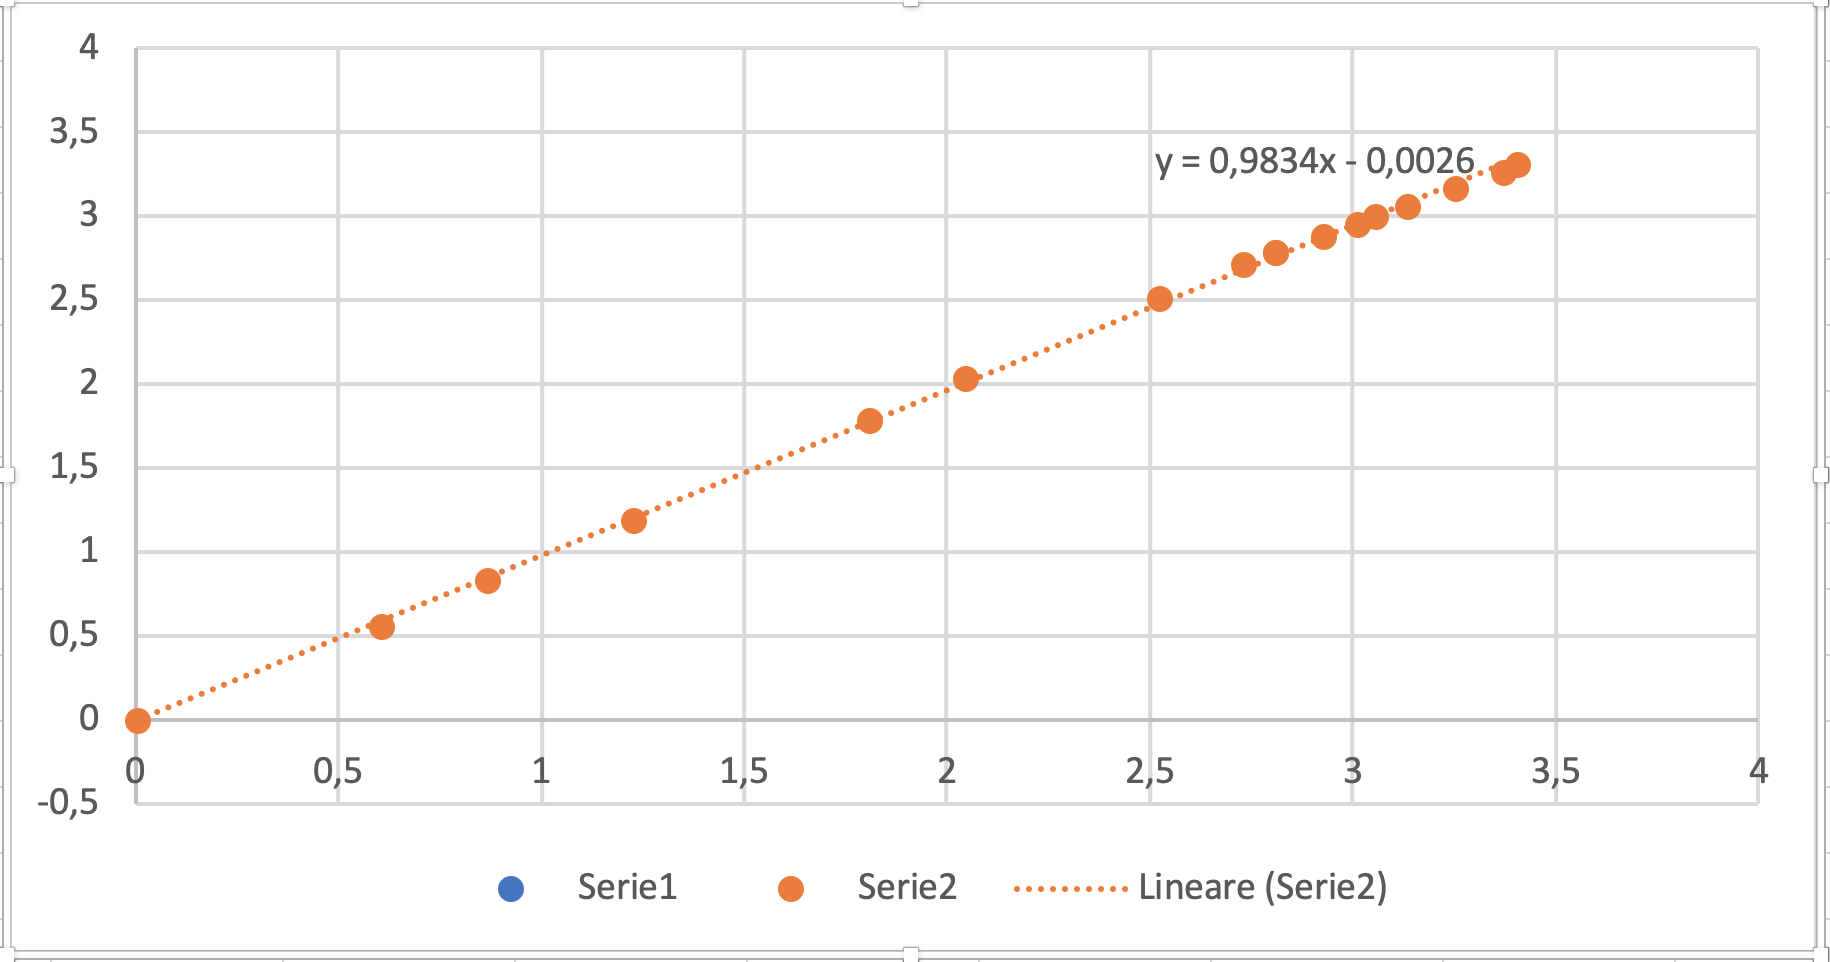
\includegraphics[width=\textwidth]{correzione_adc.png}
La relazione usata è 
\begin{equation}
    V_{corretto}=0.9834\,V_{adc}+0.0026
\end{equation}
\section{Orologio, progetto personale}
Mantenendo le stesse configurazioni adottate nell'esperienza del display e del termometro si è deciso per sperimentare le funzionalità del micro e per sfruttare il display di scrivere un programma per un orologio da polso con delle funzionalità base. L'applicativo prevede 4 sezioni:
\begin{itemize}
    \item Orologio
    \item Termometro
    \item Cronometro
    \item Impostazioni
\end{itemize}
e l'utente può navigare tra queste sezioni attraverso il bottone e la manopola del potenziometro. 
Per quanto riguarda il termometro è stato sfruttato il codice precedentemente scritto \ref{lst:display_temp}. Invece è stato necessario sviluppare un codice per implementare le funzionalità di orologio vero e proprio. Innanzitutto si crea un vettore contenente tutte le informazioni su data e ora(int ora[]=\{2,0,1,9,1,1,2,3,1,9,2,8,0,0\};) in formato Years, Month, Day, Hours, Minutes, Seconds, questo vettore ad ogni secondo dovrà essere modificato con la funzione dedicata: ad ogni secondo aumentano i secondi, se si è raggiunto il fondo scala aumentano i minuti, se anche i minuti hanno raggiunto il fondo scala si aumentano le ore e così via fino agli anni. Chiaramente a seconda del mese il fondo scala dei giorni cambia, a gennaio si piò arrivare fino a 31 mentre a febbraio di un anno bisestile fino a 29. La funzione \textit{void incrementa()} tiene conto di tutte queste eventualità e viene riportata di seguito:
\begin{lstlisting}[caption=Funzione incrementa(),language=C]
void incrementa(){
	if(ora[13]==9){
		//cifra meno significativa dei secondi
		ora[13]=0;
		//aumento ora[12]
		if(ora[12]==5){
			//cifra piu significativa dei secondi
			ora[12]=0;
			//aumento ora[11]
			if(ora[11]==9){
				//cifra meno significativa dei minuti
				ora[11]=0;
				//aumento ora[10]
				if(ora[10]==5){
					//cifra piu significativa dei minuti
					ora[10]=0;
					//aumento di un'ora
					hour=ora[9]+ora[8]*10;
					if(hour==23){
						ora[9]=0;
						ora[8]=0;
						//aumento di un giorno
						change_big_date=1;
						day=ora[7]+ora[6]*10;
						month=ora[5]+ora[4]*10;
				    year=ora[0]*1000+ora[1]*100+ora[2]*
				    10+ora[3];
						if((year%100==0 && year%400==0)||
						(year%100!=0 && year%4==0)){
							bisestile=1;
						}
						if((day==31 && (month==1|| month==3 ||
						month==5 || month==7 || month==8 ||
						month==10 || month==12))||
						(day==30 &&(month==4|| month==6 ||
						month==9 || month==11))||
						(day==28 && month==2 && !bisestile)||
						(day==29 && month==2 && bisestile)){
							ora[6]=0;
							ora[7]=1;
							//aumento il il mese
							if(month==12){
								ora[4]=0;
								ora[5]=1;
								//aumento l'anno
								year++;
								//scompongo year su ora
								ora[0]=(int)year/1000;
								resto=year%1000;
								ora[1]=(int)(resto*10)/1000;
								resto=(resto*10)%1000;
								ora[2]=(int)(resto*10)/1000;
								resto=(resto*10)%1000;
								ora[3]=(int)(resto*10)/1000;
							}
							else{
								month++;
								ora[4]=(int)month/10;
								resto=month%10;
								ora[5]=(int)(resto*10)/10;
							}
						}
						else{
							day++;
							ora[6]=(int)day/10;
							resto=day%10;
							ora[7]=(int)(resto*10)/10;
						}
					}
					else{
						hour++;
						ora[8]=(int)hour/10;
						resto=hour%10;
						ora[9]=(int)(resto*10)/10;
					}
				}
				else{
					ora[10]++;
				}
			}
			else{
				ora[11]++;
			}
		}
		else{
			ora[12]++;
		}
	}
	else{
		ora[13]++;
	}
}
\end{lstlisting}
La funzione incrementa verrà chiamata dall'interrupt dell'i2c, quando potremo trasmettere la nuova ora, ovvero ad ogni secondo. Il cronometro funzionerà in maniera del tutto analoga, ad ogni secondo verrà chiamata un'altra funzione incrementa che però è decisamente più semplice non dovendo tener conto di giorni mesi e anni bisestili. 
All'interno dell'interrupt dell'i2c dovrà essere presente una funzione per discernere cosa fare, si configurano diverse possibilità:
\begin{itemize}
    \item Trasmettere il menu
    \item Trasmettere il contenuto di una delle sezioni
\end{itemize}
Per trasmettere il menu si è proceduto nel seguente modo: aspettando che si sia finito di trasmettere il nome della prima sezione(Orologio) si legge il valore dall'adc e si confronta con dei valori di riferimento per vedere in quale delle 4 sezioni la manopola è girata. Si interpreta l'orientazione della manopola e si trasmette il titolo della sezione associata, se la manopola rimane fissa conclusa questa trasmissione non si fa nulla, altrimenti periodicamente si cambia il titolo. Per entrare in una delle sezioni si preme il tasto blu(quello dedicato agli utenti). A questo punto la funzione dell'i2c trasmetterà il contenuto della sezione opportuno. 
La sezione impostazioni funziona in maniera simile a quella del menu. Essa è adibita ad impostare l'ora e il giorno dell'orologio, quindi per velocizzare il processo si è pensato di sfruttare la manopolina per far selezionare all'utente la cifra desiderata. Ovvero partendo dalla cifra più significativa degli anni l'utente ruoterà la manopolina, a seconda di quanto viene ruotata sul display viene fatta vedere la cifra corrispondente(da 0 a 9) e premendo il pulsante si passa alla cifra successiva fino ad arrivare alla fine dove viene chiesta la conferma all'utente, girando la manopola tutta a sinistra e premendo il tasto viene confermata l'operazione, girandola a destra e premendo si ripete.
\begin{lstlisting}[caption=Porzione codice impostazioni, language=C]
else if(menu==1 && sezione==3){
		if(!trasmesso){
			i2c_loops=10;
				while(i2c_loops>0){
				TIM7->SR=0;
				TIM7->CNT=0;
				TIM7->CR1|=TIM_CR1_CEN;
				while(TIM7->SR==0){}
				i2c_loops--;
				}
				TIM7->CR1&=~TIM_CR1_CEN;
				
				switch(j){
					case(16):
						I2C1->ICR |= I2C_ICR_STOPCF; 
					I2C1->CR2 &= ~I2C_CR2_RD_WRN;
					I2C1->CR2 &= ~0xFF; 
					I2C1->CR2 |= LCD_ADDRESS; 
					NBYTES = (2 <<16); 
					char_da_trasmettere=2;
					I2C1->CR2 &= ~(0xFF<<16); 
					I2C1->CR2 |= NBYTES;
					I2C1->CR2 |= I2C_CR2_START; 
					j++;
					case(17):
						I2C1->TXDR=0x00;
						j++;
						char_da_trasmettere--;
						break;
					case(18):
						I2C1->TXDR=0x01;
						j++;
						char_da_trasmettere--;
						break;
					case(19):
						if((I2C1->ISR & I2C_ISR_STOPF)!=0){
						char_da_trasmettere=2;
						I2C1->ICR |= I2C_ICR_STOPCF; 
						I2C1->CR2 |= I2C_CR2_START; 
						j++;}
						break;
					case(20):
						I2C1->TXDR=0x00;
						j++;
						char_da_trasmettere--;
						break;
					case(21):
						I2C1->TXDR=0x02;
						j++;
					char_da_trasmettere--;
						break;
				
				case 22:
					I2C1->ICR |= I2C_ICR_STOPCF;
					I2C1->CR2 &= ~I2C_CR2_RD_WRN;
					I2C1->CR2 &= ~0xFF; 
					I2C1->CR2 |= LCD_ADDRESS; 
					NBYTES = ((lenght_da_trasmettere+3) <<16); 
					char_da_trasmettere=lenght_da_trasmettere+3;
					I2C1->CR2 &= ~(0xFF<<16); 
					I2C1->CR2 |= NBYTES;
					I2C1->CR2 |= I2C_CR2_START;
					j++;
					break;
				case 23:
					I2C1->TXDR = 0x80;
					j++;
					char_da_trasmettere--;
					break;
				case 24:
				 I2C1->TXDR = 0x80;
				 j++;
					char_da_trasmettere--;
				 break;
				case 25:
				 I2C1->TXDR = 0x40; 
				 j++;
				char_da_trasmettere--;
				 break;

				case 26:
				 if(i<lenght_da_trasmettere){
						I2C1->TXDR = *(puntatore+i);
						i++;
					 char_da_trasmettere--;
				 }
				 else{
						j++;
					 trasmesso=1;
				 }
				 break;
			 }
		}
		else if(trasmesso){
			if(loaded==1){
				if(numero_adc!=numero_precedente){
					switch(numero_adc){
						case(0):
							puntatore=num+0;
							lenght_da_trasmettere=1;
							break;
						case(1):
							puntatore=num+1;
							lenght_da_trasmettere=1;
							break;
						case(2):
							puntatore=num+2;
							lenght_da_trasmettere=1;
							break;
						case(3):
							puntatore=num+3;
							lenght_da_trasmettere=1;
							break;
							case(4):
							puntatore=num+4;
							lenght_da_trasmettere=1;
							break;
								case(5):
							puntatore=num+5;
							lenght_da_trasmettere=1;
							break;
									case(6):
							puntatore=num+6;
							lenght_da_trasmettere=1;
							break;
						case(7):
							puntatore=num+7;
							lenght_da_trasmettere=1;
							break;
							case(8):
							puntatore=num+8;
							lenght_da_trasmettere=1;
							break;
								case(9):
							puntatore=num+9;
							lenght_da_trasmettere=1;
							break;
					}
					i=0;
					j=16;
					
					trasmesso=0;
					numero_precedente=numero_adc;
				}
				loaded=0;
			}
			else if(loaded==0){
				I2C1->CR1&=~I2C_CR1_RXIE;
				I2C1->CR1&=~I2C_CR1_TXIE;
				I2C1->CR2&=~I2C_CR2_AUTOEND;
				I2C1->CR1&=~I2C_CR1_STOPIE;
				ADC1->IER|=ADC_IER_EOCIE;
				ADC1->CR|=ADC_CR_ADSTART;
				loaded=1;
			}
		}
	}
\end{lstlisting}
È stata presa una precauzione se l'interrupt del bottone o dell'adc interrompesse la trasmissione di un messaggio, salvando il numero di caratteri che si deve ancora trasmettere. Nel caso si debba trasmettere un nuovo messaggio e siano rimasti dei caratteri vecchi da mandare si mandano caratteri a caso per poi cancellare e mandare il messaggio che si vuole mandare. 
Qui di seguito viene riportato il codice per il menu
\begin{lstlisting}[caption=Menu, language=C]
switch(menu){
	case(1):
		//faccio il display dei menu
		menu=0;
		loaded=0;
		trasmesso=0;
		j=16;
		scelta_precedente=0;
		puntatore=menu_1;
		lenght_da_trasmettere=8;
		i=0;
		i2c_loops=0;
		status=0;
		break;
	case(0):
		menu=1;
		sezione=scelta_adc;
		i2c_loops=0;
		switch(sezione){
			case(0):
				msg_2[0]=ora[6]+'0';
				msg_2[1]=ora[7]+'0';
				msg_2[3]=ora[4]+'0';
				msg_2[4]=ora[5]+'0';
				msg_2[6]=ora[0]+'0';
				msg_2[7]=ora[1]+'0';
				msg_2[8]=ora[2]+'0';
				msg_2[9]=ora[3]+'0';
				puntatore=msg_2;
				lenght_da_trasmettere=10;
				j=16;
				i=0;
				break;
			case(1):
				i=0;
				j=16;
                break;
			case(3):
				loaded=0;
				trasmesso=0;
				j=16;
				numero_precedente=0;
				puntatore=num;
				lenght_da_trasmettere=1;
				i=0;
				i2c_loops=0;
				status=1;
                break;
		}
		break;
}
\end{lstlisting}

\section{Campionamento con ADC}
Questa esperienza serve a comprendere il campionamento dell'adc come può avvenire in un qualsiasi esperimento di fisica. È stato quindi abilitato l'adc con il timer 1 come trigger(ad ogni overflow del timer1 l'adc, se è pronto, converte). È stata anche abilitata la usart2 per il trasferimento dei dati campionati. 
Si configurano due possibilità per svolgere queste esperienza, ogni volta che viene convertito un dato lo si trasmette al computer, oppure si memorizzano N dati in un vettori e poi li si spedisce. 
Dipende tutto dalle esigenze dell'esperimento, usando la prima configurazione si ha il collo di bottiglia dell'usart2 ad ogni campionamento dovendo aspettare 1ms(~10 bit da mandare con velocità 9600bit/s), quindi se si vuole campionare bene un segnale a frequenze estremamente elevate essendo necessario avere una frequenza almeno doppia per il campionamento impedisce di avere segnali con frequenze maggiori di 500Hz. Nel codice seguente è stata adottata la seconda configurazione. 
A differenza di quando l'adc veniva triggerato solo via software qui si può usare anche il timer1 attraverso il suo CEN(counter enable). 
\begin{lstlisting}[caption=Interrupt ADC, language=C]
if((ADC1->ISR & ADC_ISR_ADRDY)!=0){
        //resetto l'arddy
        ADC1->ISR|=ADC_ISR_ADRDY;
        ADC1->CR|=ADC_CR_ADSTART;
}
if((ADC1->ISR & ADC_ISR_EOC) == ADC_ISR_EOC){
    if((ADC1->CHSELR & ADC_CHSELR_CHSEL0)!=0){
	    //leggo dal registro ADC_DR
        m=ADC1->DR;
        if(j<size){
            //aggiungo a small_values
            values[j]=(uint32_t)m;
            j++;
        }
        else{
            //ho finito di campionare
            ADC_CC=1;//adc conversion complete
            return;
        }
    }
    else{
        //leggo il dato per la calibrazione
        vrefint_data=ADC1->DR;
        ADC1->CHSELR&=~ADC_CHSELR_CHSEL17;
        ADC1->CHSELR|=ADC_CHSELR_CHSEL0;
        ADC1->CR|=ADC_CR_ADSTART;
    }
}
TIM1->CR1&=~TIM_CR1_CEN;
TIM1->CNT=0;
TIM1->CR1|=TIM_CR1_CEN;
\end{lstlisting}
All'interno dell'interrupt della usart2 bisogna trasmettere tutti i dati letti, si inizia nel main trasmettendo il valore vrefint letto dalla memoria, successivamente viene mandata la tensione letta al channel 17, e poi a cascata tutti i valori del segnale. Il formato dei dati mandati è un numero che va da 0 a 4095(0,FFF), separati da una newline. 
\begin{lstlisting}[caption=Interrupt USART2, language=C]
if((USART2->ISR & USART_ISR_TC) == USART_ISR_TC){
		//resetto il flag
		USART2->ICR |= USART_ICR_TCCF;
		//allora ho appena finito di trasmettere
		
			//trasmetto valore
			i++;
			if(i<lenght_da_trasmettere){
				USART2->TDR=*(puntatore+i);
			}
			else{
				if(j==-2){
						j++;
						m=vrefint_data;
				}
				else if(j<size-1){
						j++;
						m=values[j];
				}
				else{
					i=0; 
					return;
				}
				
				m_1=1000;
				msg[0]=(int)(m/m_1)+'0'; //m prima cifra
				resto=(m)%m_1;//resto
				msg[1]=(int)(resto*10/m_1)+'0';//seconda cifra
				resto=(resto*10)%m_1;//resto
				msg[2]=(int)(resto*10/m_1)+'0';//m terza cifra
				resto=(resto*10)%m_1;
				msg[3]=(int)(resto*10/m_1)+'0';//quarta
				puntatore=msg;
				USART2->TDR=*puntatore;
				i=0;
			}
	}
\end{lstlisting}
È stato scritto un piccolo script in python per la conversione dei dati raccolti in un file dall'hyperterminal. 
\begin{lstlisting}[caption=script.py,language=Python]
with open("dati_seriale.txt","r") as file:
    line=file.readline()
    cnt=1
    while line:
        if line!='\n':
            a=int(line)
            b=3.3*a/4095
            print("Line{}: {}".format(line.strip(),b))
        line=file.readline()
        cnt+=1
\end{lstlisting}
\end{document}